\documentclass[12pt, letterpaper]{article}
\usepackage{listings}
\usepackage{xcolor}
\usepackage{amssymb}
\usepackage{amsmath}
\usepackage{graphicx}
\usepackage{hyperref}
\usepackage{url}
\usepackage{float}
\usepackage{tikz}

\emergencystretch=3em
\Urlmuskip=0mu plus 1mu

% --- Style pendukung ilustrasi TikZ Neural Network ---
\definecolor{mygreen}{RGB}{0,140,80}
\definecolor{myblue}{RGB}{0,90,160}
\definecolor{myred}{RGB}{180,0,0}

\tikzset{
    nnnode/.style={circle, draw, minimum size=0.8cm, inner sep=0pt},
    nnconnect/.style={-, thick, gray},
}

% --- Konfigurasi Warna dan Style ---
\definecolor{codegreen}{rgb}{0,0.6,0}
\definecolor{codegray}{rgb}{0.5,0.5,0.5}
\definecolor{codepurple}{rgb}{0.58,0,0.82}
\definecolor{backcolour}{rgb}{0.95,0.95,0.92}

\lstdefinestyle{mystyle}{
    backgroundcolor=\color{backcolour},
    commentstyle=\color{codegreen},
    keywordstyle=\color{magenta},
    numberstyle=\tiny\color{codegray},
    stringstyle=\color{codepurple},
    basicstyle=\ttfamily\footnotesize,
    breakatwhitespace=false,
    breaklines=true,
    captionpos=b,
    keepspaces=true,
    numbers=left,
    numbersep=5pt,
    showspaces=false,
    showstringspaces=false,
    showtabs=false,
    tabsize=2,
    language=Python
}

\lstset{style=mystyle}

\title{Bagaimana \textit{Physics-Informed Neural Networks} (PINNs) bekerja?}
\author{Fajar Adie Santosa (\href{https://www.instagram.com/debug_stack/}{@debug.stack})}
\date{\today}

\begin{document}
\maketitle

\newpage
\tableofcontents
\newpage

% ============================================================
\section{Pengertian PINNs}
% ============================================================

\textit{Physics-Informed Neural Networks} (PINNs) adalah metode yang
menggabungkan \textit{neural network} dengan pengetahuan tentang hukum fisika atau persamaan diferensial. Pada
\textit{neural network} biasa, model belajar dengan melihat banyak pasangan data
masukan dan keluaran. PINNs tidak hanya belajar dari data, tetapi juga belajar
dari persamaan diferensial yang menjelaskan perilaku sistem \cite{matlab}.

Secara sederhana, \textit{neural network} pada PINNs berperan sebagai fungsi pendekatan atau \textit{approximation function}.
Misalnya, jika solusi yang ingin dicari adalah perpindahan benda terhadap waktu
$u(t)$, \textit{neural network} menerima waktu $t$ sebagai masukan dan menghasilkan perkiraan
perpindahan $\hat{u}(t)$ sebagai keluaran. Nilai keluaran ini belum tentu benar
pada awal pelatihan. Oleh karena itu, PINNs memeriksa apakah $\hat{u}(t)$
memenuhi persamaan diferensial, syarat awal, dan syarat batas dari masalah yang
sedang diselesaikan.

Untuk melakukan pemeriksaan tersebut, PINNs perlu menghitung turunan dari
keluaran \textit{neural network} terhadap masukannya. Pada contoh perpindahan, turunan pertama
$d\hat{u}/dt$ menyatakan kecepatan dan turunan kedua
$d^2\hat{u}/dt^2$ menyatakan percepatan. Turunan-turunan ini dihitung
menggunakan \textit{Automatic Differentiation} (AD).
AD berbeda dengan pendekatan beda hingga yang memperkirakan turunan dari
selisih nilai pada beberapa titik. AD menghitung turunan berdasarkan struktur
fungsi \textit{neural network}, sehingga diperlukan proses optimasi atau proses \textit{backpropagation}. Hasil turunan tersebut
kemudian dimasukkan ke persamaan diferensial. Sebagai contoh, untuk osilator
harmonik teredam, PINNs membentuk residual
\begin{equation}
    \mathcal{R}(t)
    =m\frac{d^2\hat{u}}{dt^2}
    +\mu\frac{d\hat{u}}{dt}
    +k\hat{u}(t).
\end{equation}
Apabila residual belum mendekati nol, parameter \textit{neural network} (bobot dan bias) diperbarui agar nilai residual semakin kecil.

Ketidaksesuaian antara prediksi dan hukum fisika disebut \textit{residual}. Residual dimasukkan ke dalam fungsi \textit{loss}. Jika
residual masih besar, berarti prediksi masih banyak melanggar persamaan fisika. Proses pelatihan mengubah bobot dan bias agar nilai
\textit{loss} semakin kecil. Dengan cara ini, diarahkan untuk menghasilkan fungsi yang mendekati solusi persamaan diferensial.

Keunggulan PINNs adalah kemampuannya belajar ketika data pengamatan hanya tersedia dalam jumlah sedikit atau bahkan tidak tersedia di seluruh domain. Persamaan diferensial memberikan informasi tambahan tentang bentuk solusi. Meskipun demikian, hasil PINNs tetap merupakan solusi pendekatan, sehingga akurasinya perlu diperiksa melalui residual, syarat batas, dan data pembanding jika tersedia.

PINNs dapat digunakan untuk:
\begin{itemize}
    \item Mencari pendekatan solusi persamaan diferensial biasa (PDB) dan
          persamaan diferensial parsial (PDP).
    \item Menggabungkan data pengamatan yang terbatas dengan hukum fisika.
    \item Menyelesaikan \textit{inverse problems}, seperti estimasi parameter
          fisika yang belum diketahui berdasarkan data pengamatan.
\end{itemize}

\begin{figure}[H]
    \centering
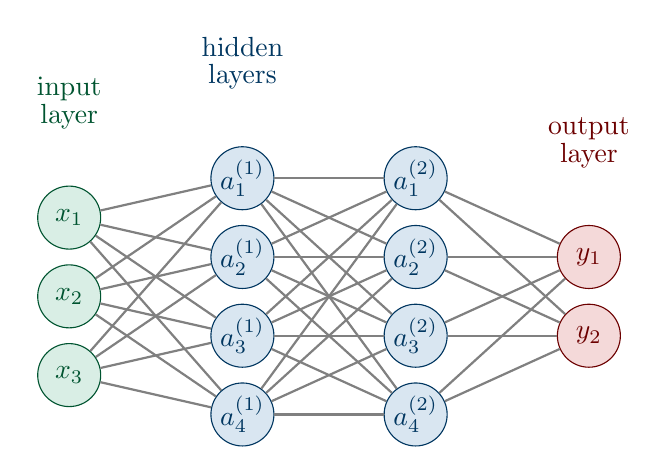
\begin{tikzpicture}[x=2.2cm,y=1.0cm]
  % Layer 1: input (3 node)
  \foreach \i in {1,...,3}{
    \pgfmathsetmacro{\y}{3/2-\i+0.5}
    \node[nnnode, mygreen!60!black, draw=mygreen!60!black, fill=mygreen!15]
      (N1-\i) at (1,\y) {$x_{\i}$};
  }
  % Layer 2: hidden pertama (4 node)
  \foreach \i in {1,...,4}{
    \pgfmathsetmacro{\y}{4/2-\i+0.5}
    \node[nnnode, myblue!60!black, draw=myblue!60!black, fill=myblue!15]
      (N2-\i) at (2,\y) {$a_{\i}^{(1)}$};
    \foreach \j in {1,...,3}{
      \draw[nnconnect] (N1-\j) -- (N2-\i);
    }
  }
  % Layer 3: hidden kedua (4 node)
  \foreach \i in {1,...,4}{
    \pgfmathsetmacro{\y}{4/2-\i+0.5}
    \node[nnnode, myblue!60!black, draw=myblue!60!black, fill=myblue!15]
      (N3-\i) at (3,\y) {$a_{\i}^{(2)}$};
    \foreach \j in {1,...,4}{
      \draw[nnconnect] (N2-\j) -- (N3-\i);
    }
  }
  % Layer 4: output (2 node)
  \foreach \i in {1,...,2}{
    \pgfmathsetmacro{\y}{2/2-\i+0.5}
    \node[nnnode, myred!60!black, draw=myred!60!black, fill=myred!15]
      (N4-\i) at (4,\y) {$y_{\i}$};
    \foreach \j in {1,...,4}{
      \draw[nnconnect] (N3-\j) -- (N4-\i);
    }
  }
  % LABELS
  \node[above=0.6cm, align=center, mygreen!60!black] at (N1-1.north) {input\\[-0.2em]layer};
  \node[above=0.6cm, align=center, myblue!60!black] at (N2-1.north) {hidden\\[-0.2em]layers};
  \node[above=0.6cm, align=center, myred!60!black] at (N4-1.north) {output\\[-0.2em]layer};
\end{tikzpicture}
    \caption{Ilustrasi \textit{fully connected network} (FCN) dengan satu \textit{input layer}, dua \textit{hidden layer}, dan satu \textit{output layer}. Setiap $a_i^{(l)}$ merupakan keluaran neuron ke-$i$ pada lapisan tersembunyi ke-$l$.}
    \label{fig:neural-network}
\end{figure}

\begin{figure} [H]
  \centering
  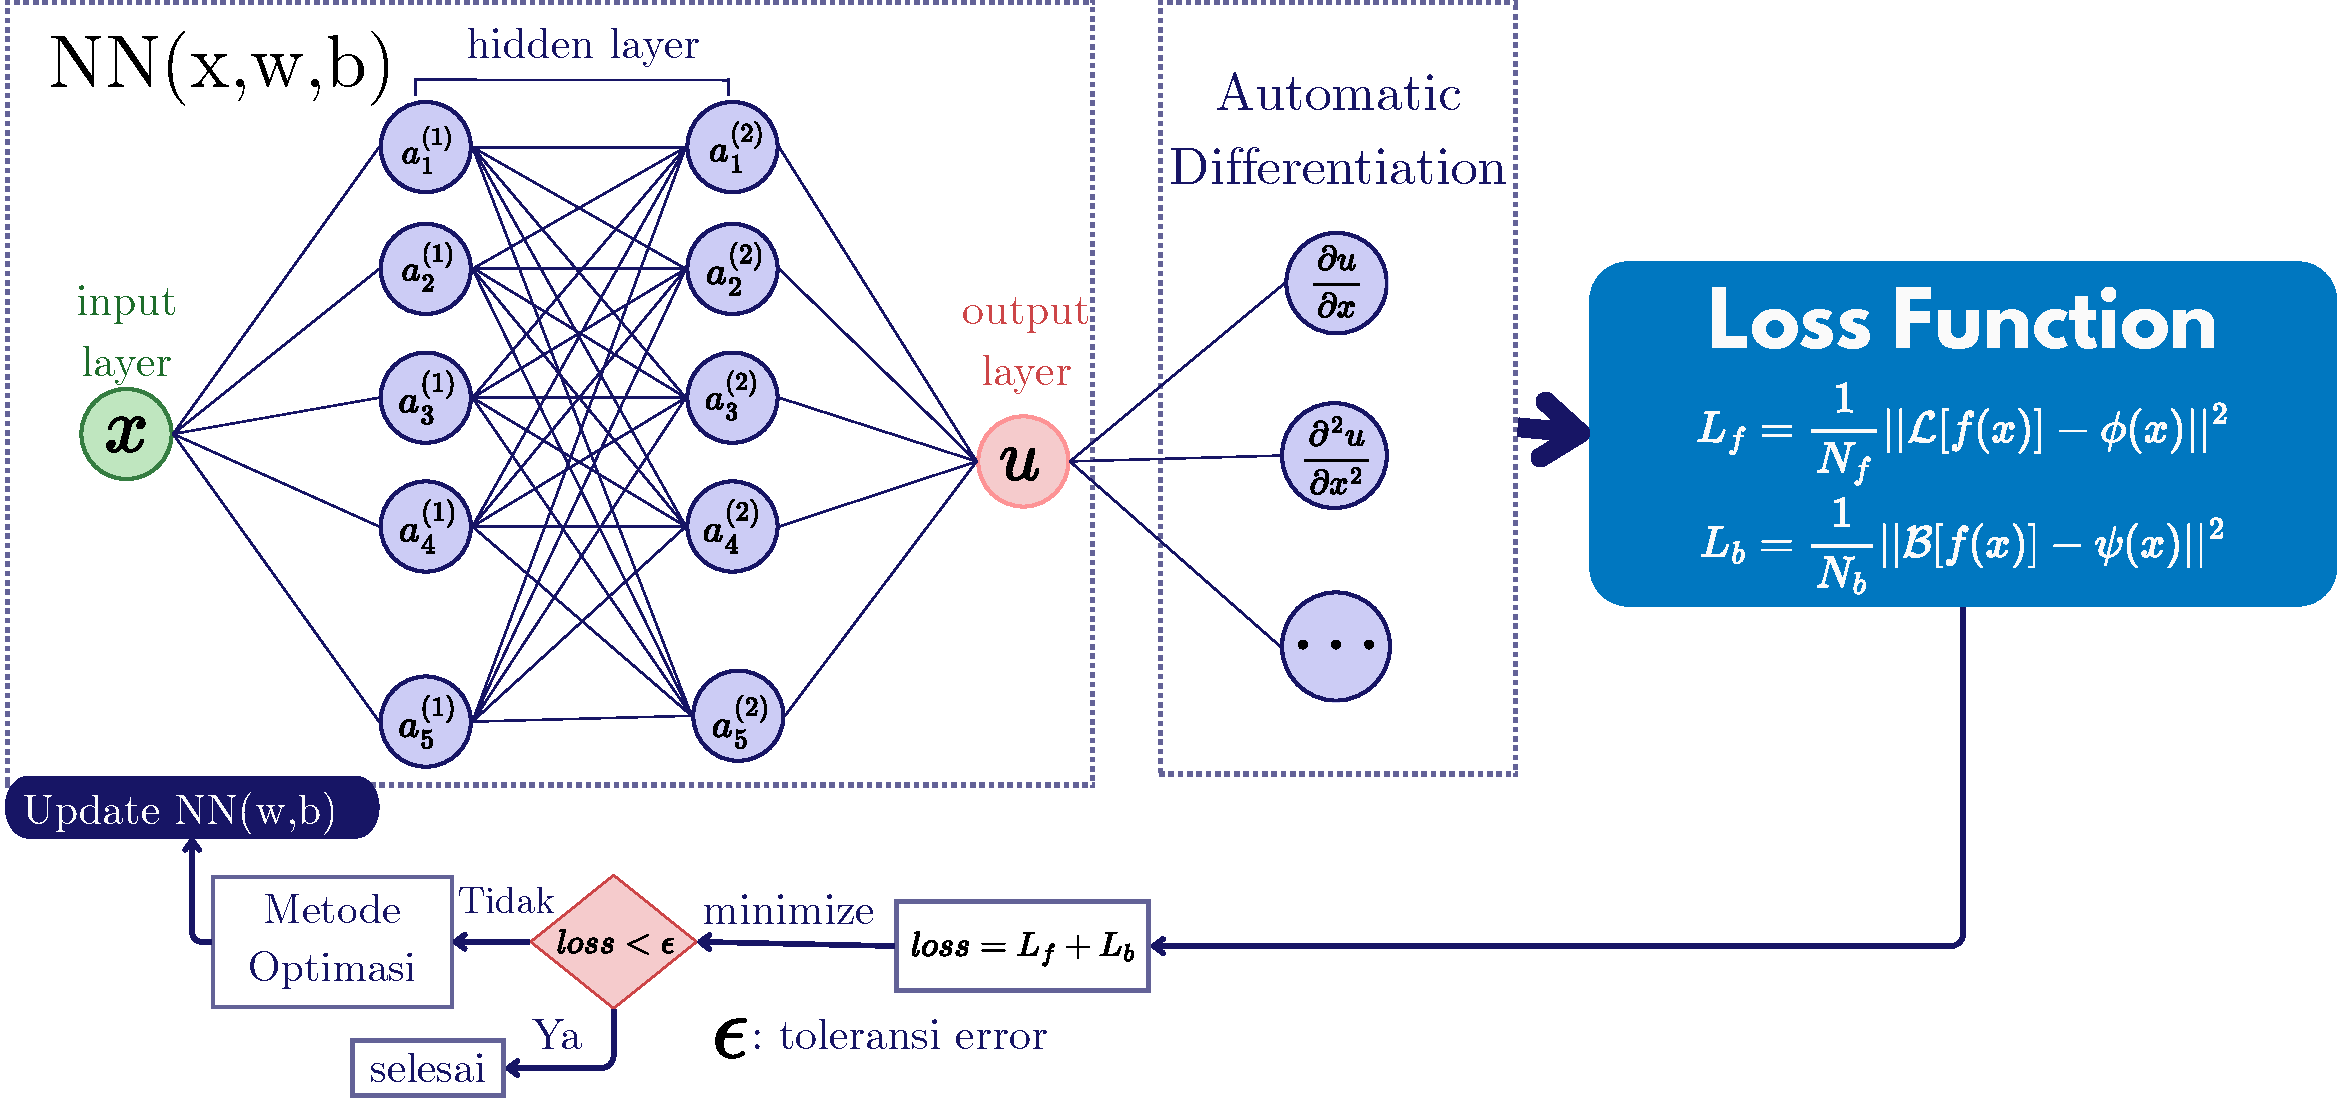
\includegraphics[width=1\textwidth]{arsitektur-pinn.pdf}
  \caption{Arsitektur PINNs}
  \label{fig:perceptron}
\end{figure}
% ============================================================
\section{Konsep Dasar PINNs}
% ============================================================

Cara kerja PINNs dapat dipahami sebagai proses menebak, memeriksa, lalu
memperbaiki solusi. Pertama, \textit{neural network} menghasilkan tebakan solusi pada
suatu masukan, misalnya posisi $x$ atau waktu $t$. Kedua, turunan dari tebakan
tersebut dihitung dan dimasukkan ke persamaan diferensial. Ketiga, hasil
pemeriksaan ini digunakan untuk memperbaiki parameter (bobot dan bias). Proses tersebut
diulang sampai residual terhadap persamaan diferensial menjadi cukup kecil.

Sebagai contoh, misalkan suatu masalah memiliki persamaan
\begin{equation}
    \frac{d^2u}{dx^2}+f(x)=0.
\end{equation}
\textit{neural network} menghasilkan pendekatan $u_{nn}(x;\theta)$, yang dimana $\theta = \{W^{(l)},b^{(l)},\dots\}$. PINNs kemudian menghitung turunan kedua \textit{neural network} dan membentuk residual
\begin{equation}
    \mathcal{R}(x)=\frac{d^2u_{nn}}{dx^2}+f(x).
\end{equation}
Jika $\mathcal{R}(x)$ mendekati nol pada banyak titik di dalam domain, berarti
prediksi \textit{neural network} semakin sesuai dengan persamaan tersebut.

\subsection{Arsitektur Neural Network}
Andaikan $u_{nn}(x;\theta)$ merupakan keluaran dari \textit{neural network}
dengan parameter $\theta$. Parameter $\theta$ mewakili seluruh bobot dan bias
yang dapat diubah selama pelatihan/\textit{training}. Secara umum, PINNs menggunakan arsitektur
\textit{fully connected network} (FCN) dengan fungsi aktivasi $\tanh$:
\begin{equation}
    u_{nn}(x;\theta) = W^{(L)} \sigma(W^{(L-1)} \cdots \sigma(W^{(1)} x + b^{(1)}) \cdots + b^{(L-1)}) + b^{(L)}
\end{equation}
di mana $W^{(i)}$ dan $b^{(i)}$ masing-masing adalah bobot dan bias pada lapisan ke-$i$,
dan $\sigma$ adalah fungsi aktivasi. Aktivasi $\tanh$ sering digunakan karena
bersifat halus dan dapat diturunkan berulang kali. Sifat ini penting karena
residual persamaan diferensial dapat memerlukan turunan pertama, kedua, atau
turunan dengan orde yang lebih tinggi.

\subsection{Menerapkan Syarat Batas dan Syarat Awal}

Fungsi \textit{loss} yang hanya memuat residual persamaan diferensial, seperti pada persamaan sebelumnya, belum menjamin solusi memenuhi syarat batas atau syarat awal dari
masalah yang diselesaikan. Residual persamaan diferensial hanya mengukur seberapa konsisten
$u_{nn}(x;\theta)$ terhadap persamaan diferensial di titik-titik kolokasi
bagian dalam domain, sedangkan syarat batas dan syarat awal merupakan
informasi tambahan yang berlaku pada titik-titik tertentu, misalnya $x=a$,
$x=b$, atau $t=0$. Tanpa mekanisme khusus, \textit{neural network} dapat saja
menghasilkan fungsi yang residual persamaan diferensialnya kecil di seluruh domain, tetapi nilainya tidak sesuai dengan syarat batas maupun syarat awal yang diinginkan.
Oleh karena itu, PINNs memerlukan cara untuk memasukkan informasi syarat
batas dan syarat awal ke dalam proses pelatihan.

Terdapat dua pendekatan umum yang digunakan untuk tujuan ini, yaitu
\textit{hard constraint} dan \textit{soft constraint}. Pada \textit{hard
constraint}, keluaran \textit{neural network} dimodifikasi secara aljabar sedemikian rupa
sehingga syarat batas atau syarat awal otomatis terpenuhi untuk nilai
parameter $\theta$ berapa pun, sehingga tidak perlu ditambahkan komponen
\textit{loss} khusus untuk itu. Sebaliknya, pada \textit{soft constraint},
keluaran \textit{neural network} tidak diubah bentuknya; syarat batas maupun syarat awal
dimasukkan sebagai penalti tambahan dalam fungsi \textit{loss}, sehingga
pemenuhannya bergantung pada proses optimasi dan hanya dijamin secara
pendekatan. Kedua subbagian berikut menjelaskan masing-masing pendekatan
secara lebih rinci beserta kelebihan dan kekurangannya.

\subsection{Hard Constraint}

Untuk memastikan solusi memenuhi syarat batas atau syarat awal secara
otomatis, digunakan pendekatan \textit{hard constraint}. Solusi dibentuk sebagai:
\begin{equation}
    u_{PINN}(x;\theta) = p(x) \cdot u_{nn}(x;\theta)
\end{equation}
di mana $p(x)$ dipilih sedemikian sehingga $u_{PINN}$ secara aljabar
memenuhi syarat batas. Dengan pendekatan ini, \textit{loss} dari syarat batas
tidak perlu dimasukkan ke dalam fungsi \textit{loss} secara eksplisit.


\subsection{Soft Constraint}
Alternatif lain adalah menggunakan pendekatan \textit{soft constraint}, di mana
syarat batas dimasukkan ke dalam fungsi \textit{loss} sebagai penalti:
\begin{equation}
    \mathcal{L} = \mathcal{L}_{PDE} + \lambda_{BC}\mathcal{L}_{BC}
\end{equation}
dengan $\lambda_{BC}$ sebagai bobot penalti untuk syarat batas. Berbeda dengan
\textit{hard constraint}, keluaran \textit{neural network} tidak dipaksa memenuhi syarat batas
secara aljabar. \textit{neural network} tetap menghasilkan aproksimasi langsung
$u_{nn}(x;\theta)$, kemudian pelatihan diarahkan agar residual persamaan diferensial dan residual
syarat batas sama-sama kecil.

Misalnya untuk masalah satu dimensi dengan syarat batas Dirichlet
\begin{equation}
    u(a) = u_a, \quad u(b) = u_b,
\end{equation}
komponen \textit{boundary loss} dapat ditulis sebagai:
\begin{equation}
    \mathcal{L}_{BC}
    =
    \left|u_{nn}(a;\theta) - u_a\right|^2
    +
    \left|u_{nn}(b;\theta) - u_b\right|^2.
\end{equation}
Apabila syarat yang digunakan adalah syarat awal, bentuknya serupa, hanya saja
titik evaluasinya berada pada waktu awal. Sebagai contoh, untuk
$u(0)=u_0$ dan $u'(0)=v_0$, penalti syarat awal dapat ditulis:
\begin{equation}
    \mathcal{L}_{IC}
    =
    \left|u_{nn}(0;\theta) - u_0\right|^2
    +
    \left|\frac{d u_{nn}}{dt}(0;\theta) - v_0\right|^2.
\end{equation}
Dengan demikian, bentuk umum \textit{loss} pada PINNs dengan
\textit{soft constraint} adalah:
\begin{equation}
    \mathcal{L}
    =
    \lambda_{PDE}\mathcal{L}_{PDE}
    +
    \lambda_{BC}\mathcal{L}_{BC}
    +
    \lambda_{IC}\mathcal{L}_{IC},
\end{equation}
Nilai $\lambda$ yang terlalu kecil dapat membuat syarat batas atau syarat awal tidak terpenuhi dengan baik.

Keuntungan utama \textit{soft constraint} adalah bentuknya lebih fleksibel
karena tidak perlu merancang fungsi pembentuk seperti $p(x)$ pada
\textit{hard constraint}. Namun, syarat batas hanya dipenuhi secara pendekatan,
bukan secara eksak. Oleh karena itu, setelah pelatihan selesai, nilai
$u_{nn}$ pada titik batas tetap perlu diperiksa untuk memastikan galat syarat
batas cukup kecil.

\subsection{Fungsi Loss}

Fungsi \textit{loss} PINNs terdiri atas residual persamaan diferensial yang
dievaluasi di titik-titik kolokasi $\{x_i\}_{i=1}^{N}$:
\begin{equation}
    \mathcal{L} = \mathcal{L}_{PDE} = \frac{1}{N} \sum_{i=1}^{N} \left| \mathcal{F}[u_{PINN}](x_i) \right|^2
\end{equation}
di mana $\mathcal{F}[\cdot]$ adalah operator diferensial dari persamaan yang
diselesaikan. Apabila tidak menggunakan \textit{hard constraint}, fungsi
\textit{loss} juga mencakup residual syarat batas:
\begin{equation}
    \mathcal{L} = \mathcal{L}_{PDE} + \lambda \, \mathcal{L}_{BC}
\end{equation}

\subsection{Tahapan Kerja PINNs}

Secara umum, proses penyelesaian persamaan diferensial dengan PINNs terdiri
atas tahapan berikut:
\begin{enumerate}
    \item Menentukan persamaan diferensial, domain, serta syarat batas atau
          syarat awal dari masalah fisika.
    \item Membentuk \textit{neural network} $u_{nn}(\mathbf{x};\theta)$ sebagai
          aproksimasi solusi. Jika digunakan \textit{hard constraint}, keluaran
          \textit{neural network} terlebih dahulu dikalikan atau dijumlahkan dengan fungsi
          pembatas yang sesuai.
    \item Memilih titik kolokasi di dalam domain. Titik ini tidak harus
          memiliki label solusi karena digunakan untuk mengevaluasi residual
          persamaan diferensial.
    \item Menghitung turunan keluaran \textit{neural network} terhadap masukan menggunakan
          \textit{automatic differentiation}, kemudian menyusun residual
          $\mathcal{R}$.
    \item Meminimalkan rata-rata kuadrat residual, serta komponen \textit{loss}
          lain jika digunakan, terhadap parameter $\theta$.
    \item Mengevaluasi solusi pada titik uji dan membandingkannya dengan solusi
          analitik menggunakan metrik galat.
\end{enumerate}

% ============================================================
\section{Problem 1: Persamaan Poisson 1D}
% ============================================================

\subsection{Problem Setup}

\textbf{Persamaan Diferensial:}
\begin{equation}
    \frac{\partial^2 y}{\partial x^2} + \pi^2 \sin(\pi x) = 0, \quad x \in [-1, 1]
\end{equation}

\subsection{Syarat Batas}
\begin{equation}
    y(-1) = 0, \quad y(1) = 0
\end{equation}

\subsection{Solusi Analitik}
\begin{equation}
    y(x) = \sin(\pi x)
\end{equation}

\subsection{Loss Residual}

Andaikan $y_{nn}$ merupakan keluaran \textit{neural network}. Residual
persamaan diferensial didefinisikan sebagai:
\begin{equation}
    \mathcal{R}(x) = \frac{\partial^2 y_{nn}}{\partial x^2} + \pi^2 \sin(\pi x) \approx 0
\end{equation}
Karena menggunakan \textit{hard constraint} dengan $p(x) = 1 - x^2$, syarat
batas $y(\pm 1) = 0$ dipenuhi secara otomatis. Sehingga fungsi \textit{loss}
hanya terdiri atas residual persamaan diferensial:
\begin{equation}
    \mathcal{L} = \mathcal{L}_{PDE} = \frac{1}{N} \sum_{i=1}^{N} \mathcal{R}(x_i)^2
\end{equation}

\subsection{Arsitektur dan Optimasi}

Model yang digunakan adalah FCN dengan arsitektur $[1, 10, 10, 1]$ dan
fungsi aktivasi $\tanh$. Optimasi dilakukan menggunakan algoritma L-BFGS
dengan \textit{automatic differentiation} untuk menghitung turunan kedua
$\frac{\partial^2 y_{nn}}{\partial x^2}$ melalui \texttt{tf.GradientTape}.

\subsection{Penjelasan Kode Langkah demi Langkah}

\subsubsection{Membangun neural network dan menerapkan syarat batas}

Fungsi \texttt{build\_fcn} menerima daftar ukuran lapisan. Dua lapisan
tersembunyi menggunakan aktivasi $\tanh$, sedangkan lapisan keluaran bersifat
linear. Keluaran mentah \textit{neural network} kemudian dikalikan dengan $1-x^2$.

\begin{lstlisting}[caption={FCN dan hard constraint pada masalah Poisson}]
inputs = tf.keras.Input(shape=(layer_sizes[0],))
a = inputs

for units in layer_sizes[1:-1]:
    a = layers.Dense(units, activation='tanh',
        kernel_initializer=initializers.GlorotNormal(),
        bias_initializer='zeros')(a)

nn_out = layers.Dense(layer_sizes[-1], activation=None)(a)
constraint = layers.Lambda(lambda x: 1.0 - tf.square(x))(inputs)
outputs = layers.Multiply()([constraint, nn_out])
model = Model(inputs=inputs, outputs=outputs)
\end{lstlisting}

Pada $x=-1$ maupun $x=1$, faktor $1-x^2$ bernilai nol. Oleh sebab itu,
\texttt{model(x)} selalu memenuhi $y(-1)=y(1)=0$ untuk nilai parameter \textit{neural network}
apa pun.


\subsubsection{Menghitung residual dengan automatic differentiation}

Dua \texttt{GradientTape} yang bersarang menghitung turunan pertama dan kedua.
Opsi \texttt{watch(x)} diperlukan karena turunan yang dicari adalah terhadap
masukan $x$, bukan terhadap parameter model.

\begin{lstlisting}[caption={Residual Poisson dan loss PDE}]
def PDE(x, model):
    with tf.GradientTape(persistent=True) as tape2:
        tape2.watch(x)
        with tf.GradientTape(persistent=True) as tape1:
            tape1.watch(x)
            y_pred = model(x)
        y_x = tape1.gradient(y_pred, x)
    y_xx = tape2.gradient(y_x, x)
    return y_xx + (np.pi**2) * tf.sin(np.pi * x)

def lossPDE(model, xPDE):
    f = PDE(xPDE, model)
    return tf.reduce_mean(tf.square(f))
\end{lstlisting}

Nilai yang dikembalikan oleh \texttt{PDE} adalah $\mathcal{R}(x)$. Pelatihan
mengecilkan \texttt{mean(square(f))}, yaitu aproksimasi diskret dari
$\mathcal{L}_{PDE}$ pada titik kolokasi.

\subsubsection{Menyiapkan titik kolokasi dan melakukan optimasi}

Kode membentuk 100 titik berjarak seragam pada $[-1,1]$, kemudian membangun
arsitektur $[1,10,10,1]$. Kelas \texttt{LBFGSOptimizer} meratakan seluruh bobot
dan bias menjadi satu vektor karena \texttt{tfp.optimizer.lbfgs\_minimize}
menerima parameter dalam bentuk tersebut.

\begin{lstlisting}[caption={Titik kolokasi dan pelatihan Poisson}]
x_train = np.linspace(-1, 1, 100).reshape(-1, 1)
x_train = tf.convert_to_tensor(x_train, dtype=tf.float32)

model = build_fcn([1, 10, 10, 1])

def loss_fn(model):
    return loss(model, x_train, x_bc, y_bc)

optimizer = LBFGSOptimizer(model, loss_fn)
optimizer.minimize(max_iterations=1000)
\end{lstlisting}

Argumen \texttt{x\_bc} dan \texttt{y\_bc} tetap diteruskan ke fungsi
\texttt{loss}, tetapi tidak digunakan karena syarat batas sudah diterapkan
secara eksak oleh \textit{hard constraint}.

\subsubsection{Evaluasi solusi}

Prediksi dihitung pada 1000 titik uji dan dibandingkan dengan
$\sin(\pi x)$. Galat relatif $L^2$ menormalkan besar selisih dengan norma
solusi analitik, sehingga nilainya dapat dibandingkan tanpa bergantung langsung
pada skala solusi.

\begin{lstlisting}[caption={Evaluasi solusi Poisson}]
y_pred = model(x_test).numpy()
y_analytic = np.sin(np.pi * x_test)
l2_error = (np.linalg.norm(y_pred - y_analytic)
            / np.linalg.norm(y_analytic))
\end{lstlisting}

% ============================================================
\section{Problem 2: Persamaan Bratu 1D}
% ============================================================

\subsection{Problem Setup}

\textbf{Persamaan Diferensial:}
\begin{equation}
    \frac{d^2 u}{d x^2} + C e^{u} = 0, \quad x \in (0, 1)
\end{equation}
dengan ukuran titik kolokasi $h = \frac{1}{n}$.

\subsection{Syarat Batas}
\begin{equation}
    u(0) = 0, \quad u(1) = 0
\end{equation}

\subsection{Solusi Analitik}

Berdasarkan referensi Shahab et al. (2025), untuk nilai $C = 1$:
\begin{equation}
    u(x) = 2 \ln\!\left( \frac{\cosh(\theta)}{\cosh(\theta(1 - 2x))} \right)
\end{equation}
di mana nilai $\theta$ diperoleh dari:
\begin{equation}
    \frac{4\theta}{\sqrt{2C}} = \cosh(\theta), \quad \theta \approx 0.379291
\end{equation}

\subsection{Loss Residual}

Andaikan $\hat{u}(x;\theta)$ merupakan aproksimasi solusi yang dihasilkan oleh
PINNs. Residual persamaan Bratu didefinisikan sebagai:
\begin{equation}
    \mathcal{R}(x)
    =
    \frac{d^2 \hat{u}}{d x^2}(x;\theta)
    +
    C e^{\hat{u}(x;\theta)}
    \approx 0.
\end{equation}

Untuk masalah Bratu 1D, formulasi \textit{hard constraint} dan
\textit{soft constraint} dapat dibandingkan sebagai berikut:

\begin{center}
\begin{tabular}{|p{0.44\textwidth}|p{0.44\textwidth}|}
\hline
\textbf{Hard Constraint} & \textbf{Soft Constraint} \\
\hline
Solusi dibentuk dengan fungsi pembatas:
\[
    \hat{u}(x;\theta) = x(1-x)u_{nn}(x;\theta).
\]
Karena $x(1-x)=0$ pada $x=0$ dan $x=1$, maka syarat batas
$u(0)=u(1)=0$ terpenuhi secara otomatis.
&
Solusi langsung diambil dari keluaran \textit{neural network}:
\[
    \hat{u}(x;\theta) = u_{nn}(x;\theta).
\]
Syarat batas tidak dipaksa secara aljabar, tetapi dimasukkan sebagai penalti
dalam fungsi \textit{loss}.
\\
\hline
Fungsi \textit{loss} hanya memuat residual persamaan diferensial:
\[
    \mathcal{L}
    =
    \mathcal{L}_{PDE}
    =
    \frac{1}{N}\sum_{i=1}^{N}\mathcal{R}(x_i)^2.
\]
&
Fungsi \textit{loss} memuat residual persamaan diferensial dan residual syarat batas:
\[
    \mathcal{L}
    =
    \mathcal{L}_{PDE}
    +
    \lambda_{BC}\mathcal{L}_{BC},
\]
dengan
\[
    \mathcal{L}_{BC}
    =
    |u_{nn}(0;\theta)|^2
    +
    |u_{nn}(1;\theta)|^2.
\]
\\
\hline
Syarat batas dipenuhi secara eksak, sehingga tidak perlu memilih bobot
\textit{loss} untuk syarat batas.
&
Syarat batas dipenuhi secara pendekatan. Nilai $\lambda_{BC}$ perlu dipilih
dengan hati-hati agar model tidak terlalu mengabaikan persamaan diferensial maupun syarat batas.
\\
\hline
\end{tabular}
\end{center}

\subsection{Arsitektur dan Optimasi}

Model yang digunakan adalah FCN dengan arsitektur $[1, 20, 20, 1]$ dan
fungsi aktivasi $\tanh$. Optimasi dilakukan menggunakan L-BFGS (\texttt{torch.optim.LBFGS})
dengan parameter \texttt{history\_size = 50} dan \texttt{line\_search\_fn = "strong\_wolfe"}.
Turunan dihitung menggunakan \textit{automatic differentiation} dari PyTorch.

\subsection{Penjelasan Kode Langkah demi Langkah}

\subsubsection{Membangun model dengan hard constraint}

Kelas \texttt{PINN} membentuk \textit{neural network} $[1,20,20,1]$. Metode
\texttt{forward} mengalikan keluaran mentah \textit{neural network} dengan $x(1-x)$ sehingga
kedua syarat batas selalu terpenuhi.

\begin{lstlisting}[caption={Arsitektur PINN untuk persamaan Bratu}]
self.net = nn.Sequential(
    nn.Linear(1, n_hidden), nn.Tanh(),
    nn.Linear(n_hidden, n_hidden), nn.Tanh(),
    nn.Linear(n_hidden, 1)
)

def forward(self, x):
    nn_out = self.net(x)
    constraint = x * (1 - x)
    return constraint * nn_out
\end{lstlisting}

Bobot dan bias lapisan terakhir dikalikan $0.01$ sebelum pelatihan. Inisialisasi
ini membuat keluaran awal mendekati nol dan membantu menjaga nilai
$\exp(u)$ agar tidak terlalu besar pada awal optimasi.

\subsubsection{Membentuk turunan dan residual Bratu}

Fungsi \texttt{derivative} menggunakan mekanisme \textit{autograd} PyTorch.
Opsi \texttt{create\_graph} diaktifkan agar grafik komputasi turunan tetap
disimpan. Dengan demikian, $u_x$ dapat diturunkan kembali untuk memperoleh
$u_{xx}$.

\begin{lstlisting}[caption={Automatic differentiation dan residual Bratu}]
def derivative(y, x):
    return torch.autograd.grad(
        y, x, grad_outputs=torch.ones_like(y),
        retain_graph=True, create_graph=True)[0]

def physics_loss(model, x, C):
    u = model(x)
    u_x = derivative(u, x)
    u_xx = derivative(u_x, x)
    f = u_xx + C * torch.exp(u)
    return torch.mean(f**2)
\end{lstlisting}

\subsubsection{Menentukan titik kolokasi dan melatih model}

Sebanyak 200 titik interior dipilih dari $h$ sampai $1-h$, dengan
$h=1/200$. Atribut \texttt{requires\_grad\_(True)} wajib diaktifkan agar
PyTorch dapat menghitung turunan solusi terhadap koordinat kolokasi.

\begin{lstlisting}[caption={Titik kolokasi dan optimizer L-BFGS untuk Bratu}]
n_col = 200
h_col = 1 / n_col
x_train = np.linspace(h_col, 1 - h_col, n_col).reshape(-1, 1)
x_train = torch.tensor(x_train, dtype=torch.float32, device=device)
x_train.requires_grad_(True)

optimizer = torch.optim.LBFGS(
    model.parameters(), max_iter=2000, max_eval=1250,
    history_size=50, tolerance_grad=1e-10,
    tolerance_change=1e-12, line_search_fn="strong_wolfe"
)
\end{lstlisting}

L-BFGS memerlukan fungsi \textit{closure} karena optimizer dapat mengevaluasi
nilai fungsi dan gradien beberapa kali dalam satu pemanggilan
\texttt{optimizer.step}. Setiap evaluasi menghapus gradien lama, menghitung
\textit{physics loss}, menjalankan \textit{backpropagation}, lalu mengembalikan
nilai \textit{loss}.

\begin{lstlisting}[caption={Closure pelatihan Bratu}]
def closure():
    optimizer.zero_grad()
    loss = physics_loss(model, x_train, C=C)
    loss.backward()
    loss_log.append(loss.item())
    return loss

loss = optimizer.step(closure)
\end{lstlisting}

\subsubsection{Mengevaluasi hasil}

Model dievaluasi pada 200 titik di $[0,1]$. Karena evaluasi tidak memerlukan
gradien, blok \texttt{torch.no\_grad()} mengurangi penggunaan memori. Prediksi
kemudian dibandingkan dengan solusi analitik menggunakan galat relatif $L^2$.

\begin{lstlisting}[caption={Evaluasi solusi Bratu}]
with torch.no_grad():
    u_pred = model(x_plot_tensor).numpy()

u_analytic = 2 * np.log(
    np.cosh(theta) / np.cosh(theta * (1 - 2 * x_plot)))
l2_error = (np.linalg.norm(u_pred - u_analytic)
            / np.linalg.norm(u_analytic))
\end{lstlisting}

% ============================================================
\section{Problem 3: Osilator Harmonik Teredam}
% ============================================================

\subsection{Dasar Fisika}

Osilator harmonik teredam dapat dimodelkan sebagai sebuah massa yang terhubung
dengan pegas dan peredam. Berdasarkan hukum II Newton, resultan gaya pegas
$-ku$ dan gaya redaman $-\mu \dot{u}$ sama dengan $m\ddot{u}$, sehingga:
\begin{equation}
    m \frac{d^2u}{dt^2} + \mu \frac{du}{dt} + ku = 0,
\end{equation}
di mana $m$ adalah massa, $\mu$ adalah koefisien redaman, dan $k$ adalah
konstanta pegas. Dengan mendefinisikan
\begin{equation}
    \delta = \frac{\mu}{2m},
    \qquad
    \omega_0 = \sqrt{\frac{k}{m}},
\end{equation}
persamaan tersebut dapat ditulis sebagai
\begin{equation}
    \frac{d^2u}{dt^2} + 2\delta\frac{du}{dt} + \omega_0^2u = 0.
\end{equation}

Energi mekanik sistem adalah
\begin{equation}
    E(t)=\frac{1}{2}m\left(\frac{du}{dt}\right)^2
         +\frac{1}{2}ku^2.
\end{equation}
Dengan mengalikan persamaan gerak dengan $du/dt$, diperoleh
\begin{equation}
    \frac{dE}{dt}=-\mu\left(\frac{du}{dt}\right)^2 \leq 0.
\end{equation}
Persamaan ini menunjukkan bahwa peredam selalu mengurangi energi sistem.
Akibatnya, amplitudo getaran mengecil terhadap waktu.

Notebook meninjau keadaan \textit{under-damped}, yaitu $\delta<\omega_0$.
Akar persamaan karakteristiknya adalah
\begin{equation}
    r_{1,2}=-\delta\pm i\omega,
    \qquad
    \omega=\sqrt{\omega_0^2-\delta^2}.
\end{equation}
Bagian imajiner menghasilkan osilasi, sedangkan bagian real negatif
$-\delta$ menghasilkan selubung amplitudo $e^{-\delta t}$.

\subsection{Syarat Awal}
\begin{equation}
    u(0) = 1, \qquad \frac{du}{dt}(0) = 0.
\end{equation}

\subsection{Solusi Analitik}

Solusi keadaan \textit{under-damped} pada notebook ditulis dalam bentuk
\begin{equation}
    u(t)=e^{-\delta t}\left(2A\cos(\phi+\omega t)\right),
\end{equation}
di mana syarat awal menentukan
\begin{equation}
    \phi=\tan^{-1}\!\left(-\frac{\delta}{\omega}\right),
    \qquad
    A=\frac{1}{2\cos\phi}.
\end{equation}
Faktor $A$ memastikan $u(0)=1$, sedangkan nilai $\phi$ memastikan
$u'(0)=0$. Pada implementasi digunakan $m=1$, $\delta=2$, dan
$\omega_0=20$. Oleh karena itu, $\mu=2\delta=4$, $k=\omega_0^2=400$, dan
domain waktu yang diamati adalah $t\in[0,1]$.

Untuk detail matematis lebih lanjut mengenai osilator harmonik teredam,
dapat dilihat pada \cite{beltoforion}.

\subsection{Formulasi PINN pada Notebook}

Berbeda dengan masalah Poisson dan Bratu, notebook osilator tidak menggunakan
\textit{hard constraint}. Aproksimasi solusi diambil langsung dari keluaran
\textit{neural network},
\begin{equation}
    \hat{u}(t;\theta)=u_{nn}(t;\theta).
\end{equation}
Pelatihan menggabungkan sejumlah kecil sampel solusi analitik dengan residual
fisika. Untuk $m=1$, residual pada titik kolokasi $t_i$ adalah
\begin{equation}
    \mathcal{R}(t_i)=
    \frac{d^2\hat{u}}{dt^2}(t_i)
    +\mu\frac{d\hat{u}}{dt}(t_i)
    +k\hat{u}(t_i).
\end{equation}
Komponen \textit{physics loss} dan \textit{data loss} masing-masing ditulis
sebagai
\begin{align}
    \mathcal{L}_{physics}
    &=\frac{1}{N_f}\sum_{i=1}^{N_f}|\mathcal{R}(t_i)|^2,\\
    \mathcal{L}_{data}
    &=\frac{1}{N_d}\sum_{j=1}^{N_d}
      |\hat{u}(t_j;\theta)-u(t_j)|^2.
\end{align}
Fungsi objektif yang benar-benar digunakan oleh kode adalah
\begin{equation}
    \mathcal{L}=\mathcal{L}_{data}
    +\lambda_{physics}\mathcal{L}_{physics},
    \qquad \lambda_{physics}=10^{-4}.
\end{equation}
Sampel data mencakup $t=0$, sehingga nilai awal perpindahan ikut diarahkan oleh
\textit{data loss}. Namun, syarat $u'(0)=0$ tidak dimasukkan sebagai komponen
\textit{loss} terpisah dan tidak dipaksakan secara aljabar. Informasi tersebut
masuk secara tidak langsung karena data pelatihan dibuat dari solusi analitik
yang telah memenuhi kedua syarat awal.

\subsection{Penjelasan Kode Langkah demi Langkah}

\subsubsection{Membangkitkan solusi analitik}

Fungsi \texttt{oscillator} menerapkan rumus solusi analitik. Perintah
\texttt{assert d < w0} memastikan parameter berada pada keadaan
\textit{under-damped}. Dalam kode, \texttt{d} menyatakan $\delta$ dan
\texttt{w0} menyatakan $\omega_0$.

\begin{lstlisting}[caption={Solusi analitik osilator harmonik teredam}]
def oscillator(d, w0, x):
    assert d < w0
    w = np.sqrt(w0**2 - d**2)
    phi = np.arctan(-d/w)
    A = 1/(2*np.cos(phi))
    cos = torch.cos(phi + w*x)
    exp = torch.exp(-d*x)
    return exp * 2 * A * cos
\end{lstlisting}

Walaupun variabel bebas pada notebook dinamai \texttt{x}, secara fisika
variabel tersebut merepresentasikan waktu $t$.

\subsubsection{Membangun neural network}

Model menggunakan tiga lapisan tersembunyi dengan 25 neuron pada setiap
lapisan dan aktivasi $\tanh$. Lapisan keluaran bersifat linear, sehingga
arsitekturnya adalah $[1,25,25,25,1]$.

\begin{lstlisting}[caption={Arsitektur neural network pada notebook osilator}]
self.net = nn.Sequential(
    nn.Linear(1, n_hidden), nn.Tanh(),
    nn.Linear(n_hidden, n_hidden), nn.Tanh(),
    nn.Linear(n_hidden, n_hidden), nn.Tanh(),
    nn.Linear(n_hidden, 1)
)

def forward(self, x):
    return self.net(x)

model = PINN(n_hidden=25).to(device)
\end{lstlisting}

Bobot dan bias lapisan keluaran selanjutnya dikalikan $0.01$. Seperti pada
masalah Bratu, langkah ini membuat prediksi awal \textit{neural network} beramplitudo kecil.

\subsubsection{Mendefinisikan data loss dan physics loss}

\textit{Data loss} mengukur kecocokan prediksi dengan sampel solusi analitik.
\textit{Physics loss} menghitung residual persamaan gerak pada titik kolokasi.
Fungsi \texttt{derivative} yang digunakan sama dengan implementasi Bratu.

\begin{lstlisting}[caption={Dua komponen loss pada osilator}]
def data_loss(model, x_data, y_data):
    yh = model(x_data)
    return torch.mean((yh - y_data)**2)

def physics_loss(model, x, mu, k):
    u = model(x)
    u_x = derivative(u, x)
    u_xx = derivative(u_x, x)
    f = u_xx + mu * u_x + k * u
    return torch.mean(f**2)
\end{lstlisting}

\subsubsection{Menyiapkan data dan titik kolokasi}

Solusi analitik dibangkitkan pada 500 titik. Ekspresi
\texttt{x[0:200:20]} mengambil 10 sampel dari bagian awal domain sebagai data
berlabel. Sementara itu, 30 titik yang tersebar pada seluruh domain dipakai
untuk mengevaluasi hukum fisika.

\begin{lstlisting}[caption={Data berlabel dan titik kolokasi osilator}]
d = 2
w0 = 20
x = torch.linspace(0, 1, 500).view(-1, 1)
y = oscillator(d, w0, x).view(-1, 1)

x_data = x[0:200:20]
y_data = y[0:200:20]
x_physics = torch.linspace(0, 1, 30).view(-1, 1)
x_physics.requires_grad_(True)
\end{lstlisting}

Pemisahan ini memperlihatkan fungsi dua jenis informasi: data berlabel
mengarahkan nilai solusi pada sebagian kecil domain, sedangkan titik kolokasi
mengarahkan bentuk solusi agar konsisten dengan persamaan diferensial pada
seluruh domain.

\subsubsection{Optimasi tahap pertama dengan Adam}

Parameter fisika dihitung dari $\delta$ dan $\omega_0$. Selama 20000
\textit{epoch}, Adam meminimalkan jumlah berbobot antara kedua komponen
\textit{loss}.

\begin{lstlisting}[caption={Pelatihan awal menggunakan Adam}]
mu = 2 * d
k = w0**2
optimizer = torch.optim.Adam(model.parameters(), lr=1e-4)
lambda_physics = 1e-4

for epoch in range(20000):
    optimizer.zero_grad()
    loss = (data_loss(model, x_data, y_data)
            + lambda_physics
            * physics_loss(model, x_physics, mu, k))
    loss.backward()
    optimizer.step()
\end{lstlisting}

Adam memberikan pembaruan parameter berbiaya relatif rendah dan digunakan
untuk membawa model menuju daerah parameter yang baik sebelum optimasi orde
kuasi-kedua.

\subsubsection{Penyempurnaan dengan L-BFGS}

Notebook kemudian menggunakan model yang sama untuk tahap L-BFGS. Dengan
demikian, tahap ini melanjutkan hasil pelatihan Adam, bukan memulai model baru.

\begin{lstlisting}[caption={Penyempurnaan solusi menggunakan L-BFGS}]
optimizer = torch.optim.LBFGS(
    model.parameters(), max_iter=10000, history_size=100,
    tolerance_grad=1e-6, tolerance_change=1e-9,
    line_search_fn="strong_wolfe"
)

def closure():
    optimizer.zero_grad()
    loss = (data_loss(model, x_data, y_data)
            + lambda_physics
            * physics_loss(model, x_physics, mu, k))
    loss.backward()
    loss_log.append(loss.item())
    return loss

loss = optimizer.step(closure)
\end{lstlisting}

\subsubsection{Mengukur galat solusi}

Setelah pelatihan, notebook menghitung MSE dan galat relatif $L^2$. MSE
mengukur rata-rata kuadrat galat titik demi titik, sedangkan galat relatif
$L^2$ membandingkan norma galat total terhadap norma solusi analitik.

\begin{lstlisting}[caption={Metrik evaluasi osilator}]
with torch.no_grad():
    u_pred = model(x)

u_analytic = oscillator(d, w0, x)
l2_error = (torch.linalg.norm(u_pred - u_analytic)
            / torch.linalg.norm(u_analytic))
MSE = torch.mean((u_pred - u_analytic)**2)
\end{lstlisting}

Plot terakhir membandingkan solusi analitik, prediksi \textit{neural network}, data berlabel,
dan lokasi evaluasi residual fisika. Plot \textit{loss} dalam skala logaritmik
digunakan untuk melihat laju konvergensi selama evaluasi optimizer.

% ============================================================
\begin{thebibliography}{99}
% ============================================================

\bibitem{matlab}
MathWorks,
\textit{Physics-Informed Neural Networks},
\href{https://www.mathworks.com/discovery/physics-informed-neural-networks.html}
{dokumentasi daring}.

\bibitem{raissi2019}
M. Raissi, P. Perdikaris, dan G. E. Karniadakis,
\textit{Physics-informed neural networks: A deep learning framework for solving forward and inverse problems involving nonlinear partial differential equations},
Journal of Computational Physics, vol. 378, hal. 686--707, 2019.
\url{https://doi.org/10.1016/j.jcp.2018.10.045}

\bibitem{lagaris1998}
I. E. Lagaris, A. Likas, dan D. I. Fotiadis,
\textit{Artificial neural networks for solving ordinary and partial differential equations},
IEEE Transactions on Neural Networks, vol. 9, no. 5, hal. 987--1000, 1998.
\url{https://doi.org/10.1109/72.712178}

\bibitem{mathworks2024}
MathWorks,
\textit{Solve Partial Differential Equations with L-BFGS Method and Deep Learning},
MATLAB Documentation, 2024.
\href{https://www.mathworks.com/help/deeplearning/ug/solve-partial-differential-equations-with-lbfgs-method-and-deep-learning.html}
{Dokumentasi daring}.

\bibitem{beltoforion}
B. Umläuft,
\textit{The Harmonic Oscillator},
beltoforion.de, diakses 2024.
\url{https://beltoforion.de/en/harmonic_oscillator/}

\end{thebibliography}

\end{document}
